\documentclass[brazil, a4paper,12pt]{article}
\usepackage[brazil]{babel}
\usepackage{graphicx}
\usepackage{geometry}
\usepackage[latin1]{inputenc}
\usepackage[T1]{fontenc}
\usepackage{url}
\usepackage{hyperref}
\usepackage{listings}
\usepackage{indentfirst}
\usepackage[usenames]{color}
\geometry{a4paper,left=3cm,right=3cm,top=2.5cm,bottom=2.5cm}


%Formatac�o de codigo fonte
\lstset{language=C,
keywordstyle=\color{red}\bf,
stringstyle=\color{red}\it,
commentstyle=\color{blue}\it,
numbers=left,
stepnumber=5,
firstnumber=1,
numberstyle=\tiny,
extendedchars=true,
breaklines=true,
captionpos=b,
tabsize=2,
frame=single,
basicstyle=\footnotesize,
showstringspaces=false
}
\renewcommand{\lstlistingname}{Programa}
\renewcommand{\lstlistlistingname}{Lista de Programas}

\begin{document}
\begin{titlepage}

  \vfill

  \begin{center}
    \begin{large}
      Universidade Federal de Juiz de Fora
    \end{large}
  \end{center}

  \begin{center}
    \begin{large}
      Instituto de Ciências Exatas 
    \end{large}
  \end{center}

  \begin{center}
    \begin{large}
      Departamento de Ciência da Computação
    \end{large}
  \end{center}

  \vfill

  \begin{center}
    \begin{Large}
	      \textbf{DCC001}\\
	      \textbf{AN�LISE E PROJETO DE ALGORITMOS}\\
	        Trabalho Pr�tico\\
    \end{Large}
  \end{center}


  \vfill

  \begin{center}
    \begin{large}
      Nome do Aluno da Silva
    \end{large}
  \end{center}

  \begin{center}
    \begin{large}
      Professor - St�nio Soares\\
    \end{large}
  \end{center}

  \vfill

  \begin{center}
    \begin{large}
      Juiz de Fora - MG \\
      \today \\
    \end{large}
  \end{center}

\clearpage
\tableofcontents 
\listoffigures
\lstlistoflistings
\listoftables
\end{titlepage}


\section{Introdu��o}

Escrever aqui a introdu��o do trabalho...

\subsection{Considera��es iniciais}

\begin{itemize}
 \item Ambiente de desenvolvimento do c�digo fonte: Code Blocks (por exemplo).
 \item Linguagem utilizada: Linguagem C.
 \item Ambiente de desenvolvimento da documenta��o: TeXnicCenter 1 BETA 7.50-Editor de \LaTeX.
\end{itemize}

\subsection{Especifica��o do problema}

Voc� dever� implementar um tipo abstrato de dados TVetor para representar vetores no espa�o $R^n$.
Esse tipo abstrato dever� armazenar a dimens�o do vetor e suas respectivas componentes. Considere que a dimens�o dos vetores ser� determinada em tempo de execu��o.


\section{Algoritmo e estruturas de dados}

Em~\cite{rp:99}, s�o apresentadas estruturas de dados...

O c�digo resultante desse processo ser� apresentado no Programa~\ref{prog:exemplo}.

\lstinputlisting[caption = {Timer},label={prog:exemplo}]{programa.c}


\section{An�lise de complexidade dos algoritmos}

A equa��o resultante da an�lise de complexidade pode ser vista na Equa��o~\ref{eq:notacao}.

\begin{equation} 
\label{eq:notacao}
O(n) = \sum_{i=1}^{n}{i^2 + 1} 
\end{equation}

Os dados coletados podem ser vistos na Tabela~\ref{tab:exemplo}

\begin{table}
 \caption{Dados referentes aos experimentos}
 \label{tab:exemplo}
 \begin{center}
  \begin{tabular}{l|ccc}
   Algoritmo & Tempo 1 & Tempo 2 & Tempo 3 \\
   \hline
   \hline
   Quicksort  &  10    &  20     &   30 \\
   HeapSort   &  10    &  60     &  530 \\
   BublleSort & 100    & 100     & 1000 \\
  \end{tabular}
 \end{center}
\end{table}



\section{Testes}

Estas estruturas s�o apresentadas na Figura~\ref{fig:exemplo}.

\begin{figure}[!ht]
	\begin{center}
		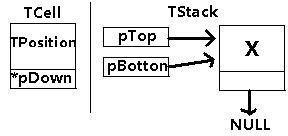
\includegraphics[width=5cm]{fig001.jpg}
	\end{center}
	\caption{Estrutura da Pilha}
	\label{fig:exemplo}
\end{figure}



\section{Conclus�o}

Neste trabalho foram revistos conceitos sobre...\cite{site1:2009}.

Muito dos algoritmos s�o extra�dos de:\cite{ziviani:2004}.

\bibliographystyle{plain}
\bibliography{modelo}

\end{document}